\chapter{Wstęp}
\label{cha:wstęp}

\section{Wprowadzenie do przetwarzania sygnałów na FPGA}
\label{sec:wprowadzenie}

\subsection{Równoległe przetwarzanie danych}
Współczesne algorytmy cyfrowego przetwarzania sygnałów (DSP) stawiają coraz wyższe wymagania wobec wydajności systemów obliczeniowych.
Tradycyjne procesory, choć rozwijają się pod względem mocy obliczeniowej, napotykają ograniczenia wynikające z sekwencyjnego przetwarzania,
co sprawia, że są mniej efektywne przy obliczeniach, które można prowadzić równolegle. W tym kontekście układy FPGA (Field-Programmable Gate Arrays) wyróżniają się
możliwością równoległego przetwarzania danych, co pozwala na znaczne przyspieszenie złożonych operacji. Dzięki takiemu rozwiązaniu można przetwarzać wiele
strumieni danych jednocześnie, co daje wyraźną przewagę nad klasycznymi procesorami, szczególnie w aplikacjach wymagających wysokiej przepustowości i małych opóźnień.

\subsection{Kontrola zegara i deterministyczne przetwarzanie}
Kolejną zaletą układów FPGA jest możliwość precyzyjnego dostosowania częstotliwości zegara do wymagań projektowych. Dzięki wykorzystaniu języków opisu sprzętu,
takich jak VHDL czy Verilog, projektant ma pełną kontrolę nad wartościami sygałów w każdym takcie zegara, co umożliwia dokładne określenie, kiedy i jakie operacje mają się odbywać.
To daje pewność, że w takich aplikacjach jak filtr FIR dane będą przetwarzane i transmitowane w równych, określonych odstępach czasowych, co jest kluczowe. W odróżnieniu od procesorów,
gdzie prędkość zegara jest sztywno ustalona, a czas wykonywania kodu może być niedeterministyczny -- szczególnie w językach wysokiego poziomu, takich jak Python -- FPGA zapewniają
pełną deterministyczność przetwarzania. Nawet w językach niskiego poziomu użytkownik nie ma pełnej kontroli nad czasem wykonywania kodu, co może prowadzić do pewnych opóźnień.)

\subsection{Platforma Cyclone V SoC}
W mojej pracy skupię się na układzie heterogenicznym firmy Intel -- Cyclone V SoC. Jest to budżetowy układ zawierający w swojej architekturze zarówno FPGA, jak i
HPS (Hard Processor System) oparty na procesorze ARM, co pozwala na rozdzielenie zadań pomiędzy obie architektury. Mimo że Cyclone V SoC nie jest układem najwyższej klasy,
jego cena oraz możliwości konfiguracyjne sprawiają, że znajduje zastosowanie w projektach wymagających kompromisu między wydajnością a kosztami. W mojej pracy pokażę, jak można
efektywnie wykorzystać ten układ do implementacji zaawansowanych algorytmów przetwarzania sygnałów.

\begin{figure}[!htb]
    \centerline{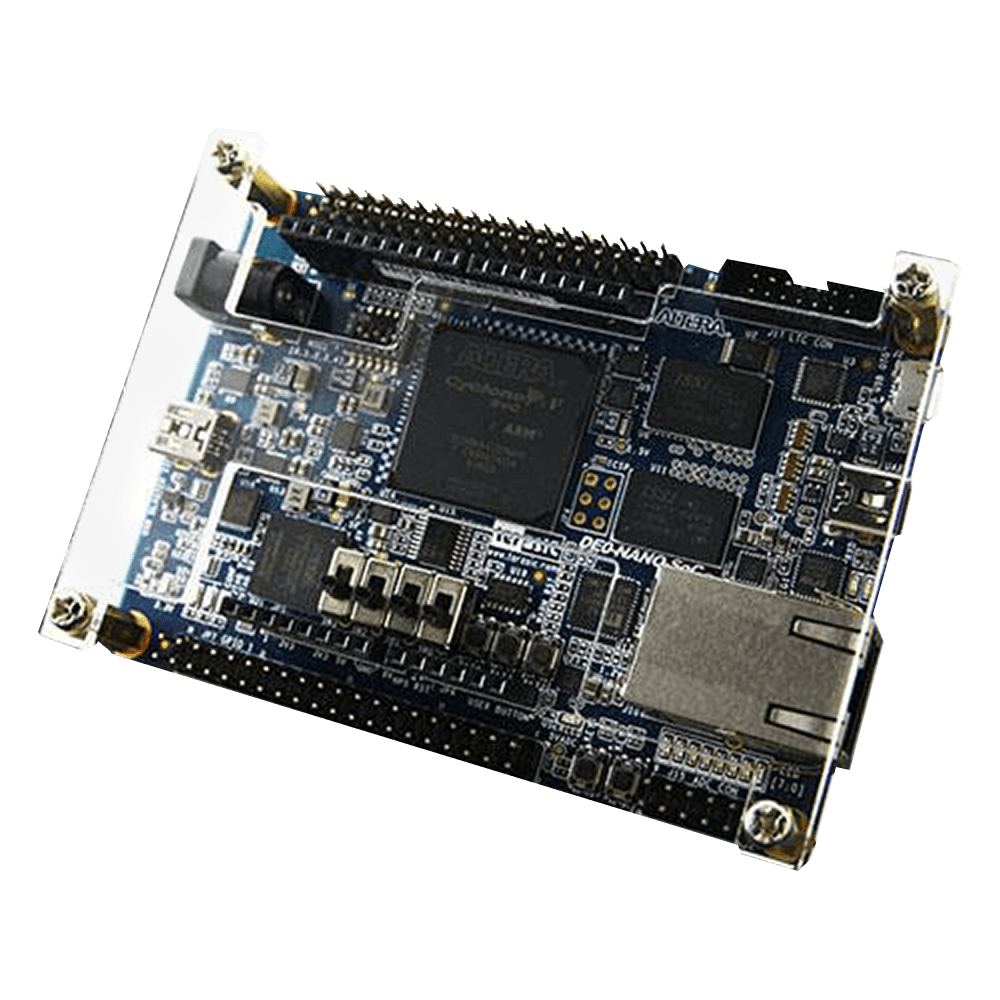
\includegraphics[scale=0.2]{de0-nano-soc.png}}
    \caption{Układ DE0-Nano-SoC (Cyclone V)}
    \label{fig:de0-nano-soc}
\end{figure}

\section{Cele pracy}
\label{sec:celePracy}
Celem pracy jest opracowanie kompleksowego systemu przetwarzania sygnałów. Część FPGA systemu będzie odpowiedzialna za implementację algorytmów DSP, w tym filtru FIR oraz modułu
realizującego dyskretną transformatę Fouriera (DFT). System ten będzie wyposażony w dwie pamięci, pomiędzy którymi dane będą transmitowane, przetwarzane, a następnie zapisywane.

Równocześnie wbudowany procesor będzie pełnił funkcję jednostki sterującej, uruchamiając serwer, który umożliwi użytkownikowi zdalną interakcję z systemem poprzez stronę internetową.
Strona będzie umożliwiać wprowadzanie danych do FPGA, inicjowanie procesów przetwarzania oraz monitorowanie wyników. Taki podział zadań na układ FPGA i HPS umożliwia
efektywną realizację złożonych algorytmów DSP, zapewniając wysoką wydajność oraz intuicyjną obsługę przez użytkownika.



















